\documentclass[a4paper,11pt]{article}
\input{/home/tof/Documents/Cozy/latex-include/preambule_lua.tex}
\newcommand{\showprof}{show them}  % comment this line if you don't want to see todo environment
\fancyhead[L]{Composition d'une image}
\newdate{madate}{10}{09}{2020}
%\fancyhead[R]{\displaydate{madate}} %\today
\fancyhead[R]{Seconde - SNT}
%\fancyhead[R]{Première - NSI}
%\fancyhead[R]{Terminale - NSI}
\fancyfoot[L]{~\\Christophe Viroulaud}
\AtEndDocument{\label{lastpage}}
\fancyfoot[C]{\textbf{Page \thepage/\pageref{lastpage}}}
\fancyfoot[R]{\includegraphics[width=2cm,align=t]{/home/tof/Documents/Cozy/latex-include/cc.png}}

\begin{document}
\begin{Form}
\begin{commentprof}
mettre couleurs.zip sur site
\end{commentprof}
\section{Problématique}
Le premier appareil photographique numérique semble avoir été commercialisé en 1981 (Sony). Depuis la photographie numérique n'a cessé de progresser pour pratiquement remplacer l'argentique aujourd'hui.
\begin{center}
\shadowbox{\parbox{10cm}{\centering Comment construire une image numérique?}}
\end{center}
\section{Les pixels}
Une image numérique est composée de carrés élémentaires nommés \textbf{pixels}. L'image n'est pas \emph{continue}.
\begin{center}
\centering
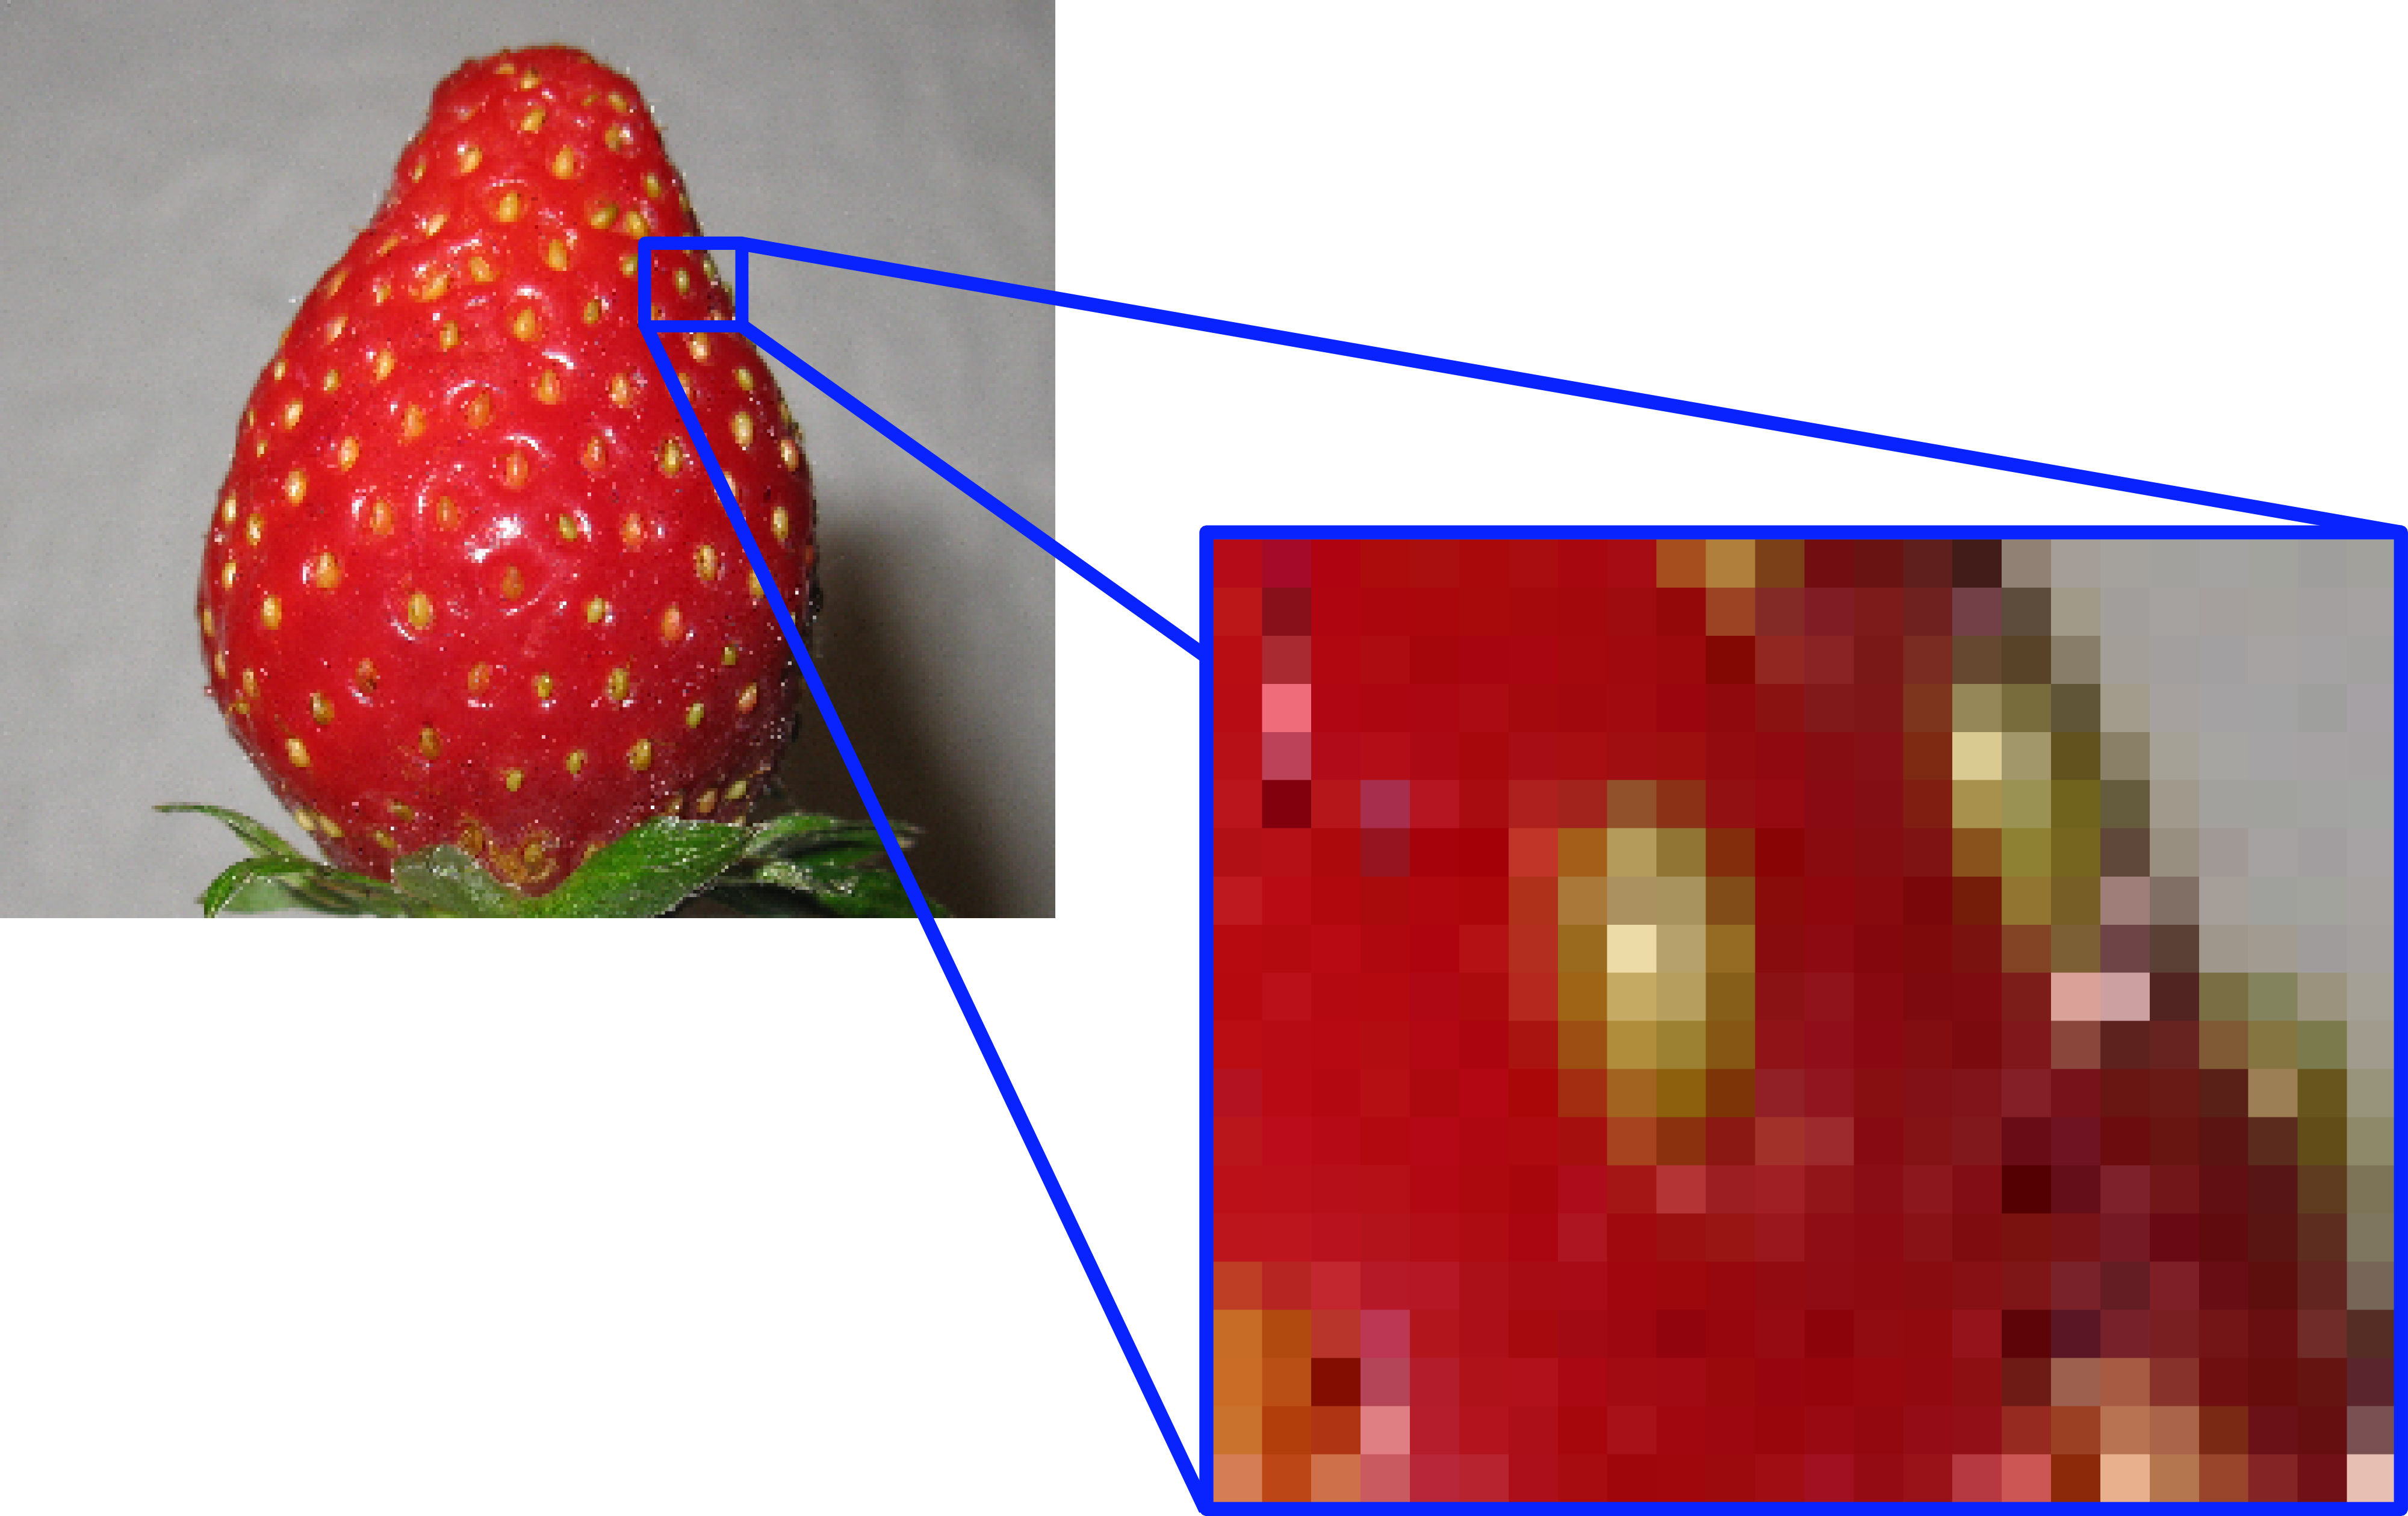
\includegraphics[width=7cm]{ressources/fraise.png}
\captionof{figure}{Agrandissement}
\label{fraise}
\end{center}

\begin{activite}
\begin{enumerate}
\item Combien de pixels composent la figure \ref{pixel}?
\begin{center}
\centering
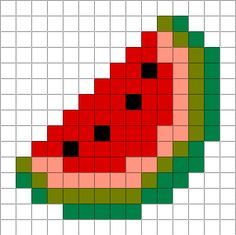
\includegraphics[width=4cm]{ressources/pasteque.jpg}
\captionof{figure}{Image pixelisée}
\label{pixel}
\end{center}
\item Dans \emph{Google Images} chercher un \emph{paysage}.
\item Cliquer une fois sur une des images; elle apparaît à droite de l'écran.
\item Passer la souris sur l'image; des nombres apparaissent dans le coin bas gauche. Que représente-t-il?
\item Combien de pixels composent cette image?
\end{enumerate}
\end{activite}

\section{Les couleurs}
\subsection{Synthèse additive}
À partir de trois sources lumineuses primaires (\emph{Rouge, Vert, Bleu - RVB ou RGB en anglais}) il est possible d'obtenir une grande variété d'autres couleurs.
\begin{activite}
\begin{enumerate}
\item Télécharger le dossier compressé \emph{couleurs.zip} sur le site \mbox{\url{https://cviroulaud.github.io}}.
\item Extraire les fichiers.
\item Ouvrir le fichier \emph{synthese-additive} avec le logiciel \emph{Gimp}.
\item Déplacer le disque vert sur le rouge. Quelle couleur obtient-on?
\item Déplacer les disques et noter les couleurs obtenues en fonction des associations. Quelle couleur obtient-on quand on superpose les trois disques?
\end{enumerate}
\end{activite}
\begin{aretenir}[]
Chaque pixel de l'écran est une association de \emph{rouge, vert, bleu}. Chacune de ces sources primaires varie entre 0 et 255.
\end{aretenir}
\begin{activite}
\begin{enumerate}
\item Se rendre sur la page \url{https://htmlcolorcodes.com/fr/}.
\item Dans le cadre de droite modifier les valeurs RGB:
\begin{itemize}
\item R 128
\item G 128
\item B 128
\end{itemize}
Quelle couleur obtient-on?
\item Utiliser maintenant la combinaison (200, 200, 200). Quelles couleurs obtient-on quand les trois valeurs sont identiques?
\item Comment obtient-on du blanc? du noir?
\item Combien de niveaux de gris peut-on réaliser?
\end{enumerate}
\end{activite}
\subsection{Synthèse soustractive}
Il existe d'autres systèmes. Une imprimante à jet d'encre utilise quatre encres: \emph{Cyan, Magenta, Jaune, Noir}. En appliquant les trois premières couleurs sur une feuille blanche il est possible de créer les autres nuances par \emph{synthèse soustractive}.
\begin{activite}
\begin{enumerate}
\item Convertir le nom des couleurs en anglais.
\item Sur le site \url{https://htmlcolorcodes.com/fr/} obtenir le noir en utilisant les couleurs Cyan, Magenta, Jaune.
\item Puisqu'il est possible d'obtenir le noir en combinant les trois couleurs, quel est l'intérêt de rajouter une cartouche d'encre noir dans l'imprimante?
\end{enumerate}
\end{activite}
\end{Form}
\end{document}